% !TEX program = pdflatex
% !TEX enableSynctex = true
% !BIB program = bibtex

\documentclass[12pt]{article}

\usepackage{setspace}
\usepackage{amsmath}
\usepackage{amsfonts}
\usepackage{graphicx}
\usepackage{float}
\usepackage{dsfont}
\usepackage{natbib}
\addtolength{\oddsidemargin}{-.7in}
\addtolength{\evensidemargin}{-.7in}
\addtolength{\textwidth}{1.4in}
\usepackage{enumerate}
\onehalfspacing
\usepackage{geometry} % Required for customizing page layout
\usepackage{ragged2e}

\usepackage{caption}
\usepackage{booktabs}

\usepackage{hyperref}
\hypersetup{
	pdfstartview = FitH,
	pdfauthor = {...},
	pdftitle = {...},
	pdfkeywords = {...; ...; ...; ...},
	colorlinks = true,
	linkcolor = blue,
	urlcolor = blue,
	citecolor = blue,
	linktocpage=true
}

\DeclareMathOperator{\E}{\mathbb{E}}
\DeclareMathOperator*{\argmax}{arg\,max}
\DeclareMathOperator*{\argmin}{arg\,min}

\title{Credit Spreads Under Heterogeneous Debt Contracts}
\date{}

\begin{document}

\author{Barnabás Székely}
\date{\today}
\vspace{-1in}

\maketitle

\begin{abstract}
\noindent

I study the credit spreads of asset-based and cash flow-based debt contracts in a heterogeneous firms model with in-equilibrium defaults. For CF-based debt contracts, an important yet under-studied determinant is the ex-ante probability that the firm would be liquidated under financial distress. This puts small businesses, which often choose liquidation, at a disadvantage. Their access to cash flow-backed debt is limited by high ex-ante liquidation probabilities, whereas their access to asset-based debt is constrained by a lack of pledgeable assets. These compounding disadvantages yield considerable misallocation of capital, that bankruptcy frameworks can mitigate by facilitating and incentivising small firm reorganizations.

\bigskip{}
\bigskip{}
%\bigskip{}
%\bigskip{}
%\vspace{-0.5cm}

Keywords: Heterogeneous firms, Credit market frictions, Cash flow-based lending, Earnings-based constraints

\medskip{}
% JEL Classification Code: E32, C22, E27.
\end{abstract}
\thispagestyle{empty}

\pagebreak{}

\section{Introduction \label{sec:introduction}} 
Corporate credit market frictions are typically characterized as borrowing constraints defined the by value of pledgeable assets. Recent research has challenged this view based on more granular analyses of corporate credit contracts. These argue that the majority of corporate debt is backed by borrowers’ future cash flows rather than assets, which implies that credit frictions are better described as borrowing constraints defined by current earnings. These results led to several contributions focused on re-assessing credit market frictions in structural analyses. \vspace{3mm} \\
However, such studies typically adopt a `no equilibrium defaults' framework,\footnote{Dating back to Kiyotaki and Moore (1997).} where lenders impose borrowing limits to such that firms always meet their debt obligations. This gives rise to `hard constraints' to borrowing. Firms that borrow against assets are constrained by the value of their collateral, whereas those borrowing against cash flows are limited by current earnings. One shortcoming of this framework is its inability to account for variations of interest rates across firms - since debt contracts are always honored, every firm faces the same risk-free rate. This directed the focus of this literature to studying the effects of debt covenants,\footnote{These are legally binding agreements imposed by the creditor on the lender, that typically take the form of hard constraints implied by the no equilibrium defaults framework.} while credit spreads received considerably less attention.  \vspace*{3mm} \\
I fill this gap in the literature by studying the determinants of credit spreads for asset-based and cash flow-based debt. This requires a model framework where a certain proportion of firms choose to file for bankruptcy each period. Moreover, debt may be backed by assets, such that lenders' in-default payments are determined by their liquidation value, or by future cash flows, such that lenders' in-default payments reflect the going-concern value of the firm. Lenders set interest rates following their exposure to default and the probability of this event. Both of these increase with debt, causing interest rates to rise with borrowing. This yields `soft borrowing constraints', specific to firms' current state, credit demand and debt financing strategy, which allows me the structural analysis of credit spreads while considering heterogeneity in debt contracts. \vspace*{3mm} \\
\textbf{Here, mention the empirical analysis and find a segway to the importance of the liquidation probability} The structural model is supported by an empirical analysis of debt US debt contracts between 2010-2023. For both type of debt, I observe a negative relationship between credit spreads and the probability of liquidation, as well as assets. This finding contradicts the predictions of `hard constraints framework' as it suggests that size and profitability are important determinants of credit market frictions regardless of the type of borrowing. \vspace{3mm} \\
Bankrupt firms may undergo liquidation or reorganization (Chapter 7 and Chapter 11 in the US bankruptcy code). In the absence of collateral, the lender may retrieve only a fraction of the borrower's liquidation value. Hence, CF-based debt is backed mainly by the belief that the borrower would produce positive cash-flows even after experiencing financial distress. Choosing liquidation in bankruptcy terminates all future cash-flows. Hence, high ex-ante probability of liquidation raises the credit spread of CF-based debt, by increasing lenders' exposure to default. Crucially, the proportion of liquidating firms decreases sharply with size. For instance, 56.6\% of firms with less than 100 million USD worth of total assets liquidate, but only 4.27\% of firms larger than this do so. I argue that in the case of CF-based debt, the value of assets serves as a proxy of liquidation probability rather than a direct determinant of in-default payments. \vspace*{3mm} \\ 
To study the impact of this trend, I consider endogenous liquidation decision in structural the model, similar to Corbae and D'Erasmo (2021). Firms in financial distress may  be liquidated, which entails exiting the market, or reorganized, which allows them to continue but incurs significant fixed costs.\footnote{These are generated by the time, legal and personnel expenses involving the renegotiation of debt \textit(cit).} This introduces economies of scale in reorganizations. Small firms are at a disadvantage under both type of debt contracts. Their access to CF-based debt is limited by high liquidation probabilities, while their access to asset based debt is limited by the amount of pledgeable assets. The model suggest that these compounding disadvantages are an important source of capital misallocation. However, bankruptcy framework that incentivise and facilitate small firm reorganization can mitigate this effect. \vspace*{3mm} \\
The paper is organized as follows. Section 2 reviews the related literature. Section 3 addresses the empirical analysis, beginning with a description of the data and the classification of debt contracts into asset-based and cash flow-based. It then presents descriptive statistics for debt contracts and firm characteristics. Lastly, it analyzes the empirical predictors of credit spreads and debt financing strategies. Section 4 introduces the structural model and section 5 discusses the results. Section 6 concludes.

\section{Literature \label{sec:literature}} 
This ppaper reflects on the contributions the highlight the prevalence of CF-based borrowin. Lian and Ma (2021) finds that majority of US corporate debt is backed by future cash flows rather than specific physical assets, which suggests that credit frictions are better described as earnings-based constraints. They support this finding by documenting the extensive use of earnings-based covenants in US corporate debt contracts. Similarly, Drechsel (2023) finds that three of the four most frequently used debt covenants limit debt based on current earnings rather than assets. \vspace{3mm} \\
These results led to the reevaluation credit frictions in macroeconomic models. Switching to earnings based constraints have been shown to have substantial impact on various model outcomes. Lian and Ma (2021) argues that this mitigates the financial acceleration driven by feedback of asset prices into credit constraints.\footnote{This mechanism was first highlighted by Bernanke, Gertler, and Gilchrist (1999).} Drechsel and Kim (2022) argues that firms subject to earnings based constraints under-borrow, while those facing asset based constraints over-borrow. Drechsel (2023) considers `investment shocks' that move the price of the capital countercyclically. He demonstrates that the effects of such shocks are heterogeneous depending on the borrowing constraint in place.  \vspace{3mm} \\
Earnings-based constraints have also been studied in relation to monetary policy, since unlike asset-based constraints, these directly interact with sticky prices. Greenwald (2019) points out interest coverage covenants, which limit borrowing in the ratio of interest payments to earnings introduce a direct channel of monetary policy transmission. Caglio, Darst and Kalemli-Ozcan (2021) studies the investment and credit channel of monetary policy when firms are backed by different type of collateral. They document that small and risky firms often rely on `going-concern value' collateral, which makes them more responsive to monetary policy shocks. \vspace{3mm} \\
The structural model proposed here adopts the heterogeneous firms framework established by Khan, Senga and Thomas (2013). This framework has been extended to study the decision to borrow against assets or cash flows. Öztürk (2023) highlights the volatility of earnings and pledgeability as important determinants of this decision. Gonzalez and Sy (2024) documents on Spanish data that reliance to CF-based borrowing (CF-based debt to total debt) is U-shaped across firms size, meaning that small and large firms borrow most against cash flows. On the other hand, empirical research such as Kermani and Ma (2020) highlight the importance of `asset specificity,' which describes how much value assets would lose under liquidation. \footnote{These papers are closely related to my research, since credit conditions and the debt financing strategy are jointly determined. Firms react to the credit conditions set by debt covenants and credit spreads by optimizing their debt financing strategy, which in turn affects the credit market frictions they eventually face.} \vspace{3mm} \\
Both Öztürk (2023) and Gonzalez and Sy (2024) adopt the `hard constraints' framework where firms choose between earnings-based or asset-based constraints based on which is less restrictive. In essence, this amounts to modelling heterogeneity in borrowing constraints. This approach does not allow for holding both types of debt simultaneously, which can be a significant limitation, since in the United States these borrowers represent a substantial share of the market. 
Conversely, I consider heterogeneity in debt contracts (differences in in-default payoffs) rather than borrowing constraints. This yields a more flexible framework that allows for firms that hold type of debt simultaneously. \vspace{3mm} \\
As mentioned above, I also consider in-equilibrium defaults and a liquidation decision similar to Corbae and D'Erasmo (2021), which implies lenders must account for the probability that the borrower would be liquidated under financial distress. However, they do not consider heterogeneity in debt contracts, meaning lenders and borrowers do not need to decide ex-ante whether the debt should be backed by assets or future cash flows. This yields more flexibility in collecting in-default payments, depending on the liquidation or reorganization decision of the firm.  \vspace{3mm} \\
Research into credit market frictions under asset-based and CF-based contracts typically focuses on the role of debt covenants, while credit spreads received considerably less attention. However, a closely related branch of empirical literature studies the role of different types of collateral in reducing credit spreads -  Cerqueiro, Ongena, Roszbach (2016), Luck and Santos (2020), Benmelech, Kumar and Rajan (2022). These studies must address endogeneity due to firms' self-selection into collateralized and uncollaterialized borrowers. They overcome this issue by using firm, bank, and time fixed effects, which yields plausible identification, but it restricts analyses to firms that borrowed both with and without collateral from the same lender within the same time period. Once its effect is adequately identified, collateral is to decrease credit spreads, but the strength of this effect varies across different types of collateral. \vspace{3mm} \\
Another related strand literature studies the role of unsecured debt in inducing investment (Biguri, 2020) or exacerbating credit cycles (Azariadis, Kaas and Wen, 2016). Moreover, Rampnini and Viswanathan (2022) studies firms' decision to borrow secured or unsecured. Note that categorizing debt as secured or unsecured is not analogous to differentiating asset-based and cash flow-based debt. The former relates to priority in bankruptcy, whereas the latter considers the economic determinants of lenders' in-default payoffs. Finally, I study the misallocation caused by the limited access to external finance. For extensive reviews of this the misallocation literature, see Restuccia and Rogerson (2012) and Hopenhayn (2014).

\section{Empirical analysis \label{sec:empirical analysis}}

This section covers the empirical analysis of debt contracts and bankruptcy processes for US non-financial corporations. Section 3.1 discusses the data and present summary statistics of firms and debt contracts. Section 3.2 details the classification of debt contracts into asset-based and CF-based debt. Section 3.3 and 3.4 presents the determinants of credit spreads. This exercise can be considered complementary to the analysis of debt covenants, therefore I highlight instances where the credit frictions implied by spreads are different from those implied by debt covenants. Finally, section 3.5 discusses the limitations of empirical analyses. 

\subsection{Descriptive statistics \label{sec:descriptive stats}}
I study a total of 113,774 debt contracts held by 6,925 non-financial corporations between 2010Q1 and 2023Q2. Debt-level data comes from S\&P's Capital IQ and firm-level data is from Compustat North America. This yields and extensive, but not representative sample of US non-financial corporations. In particular, since Compustat focuses on listed corporations, SMEs are underrepresented in the sample. Moreover, I only consider firms with at least one debt contract, so the analysis does not address borrowing decisions on the extensive margin. Moreover, I present evidence from Federal Judicial Center's Integrated Database (IDB). This contains a total of 178,256 bankruptcy filings by US-based corporations between 2010 and 2023. To be consistent with the model, only Chapter 7 or Chapter 11 filings are considered, which constitute the majority of corporate bankruptcy filings. \vspace{3mm} \\
Table 1. presents firm-level summary statistics for indicators of size, financial position, and borrowing conditions and table 2. presents debt-level summary statistics, for contract value, maturity interest rates and spreads. Credit spreads are calculated as a difference of the interest rate and the T-bill rate at the corresponding maturity.
\begin{table}[H] 
    \centering
    \resizebox{0.95\textwidth}{!}{%
    \begin{tabular}{lrrrrrr}
    \multicolumn{7}{l}{\textbf{Firm-Level Summary Statistics}} \\
    \hline
        & \textbf{Mean} & \textbf{p10} & \textbf{p25} & \textbf{Median} & \textbf{p75} & \textbf{p90} \vspace{1mm} \\
    Total Assets (millions USD) & 5235.16 & 11.39 & 73.11 & 582.60 & 2696.20 & 9567.60 \\
    Qtr. Revenue (millions USD) & 1073.75 & 0.18 & 8.77 & 109.62 & 551.79 & 1891.00 \\
    Employees (thousands) & 11.93 & 0.03 & 0.15 & 1.37 & 6.91 & 22.85 \\
    Firm Age (years) & 44.61 & 9 & 16 & 30 & 59 & 109 \\
    Cash to Assets (Liquidity) & 0.17 & 0.01 & 0.03 & 0.09 & 0.21 & 0.46 \\
    Debt to Assets (Leverage) & 0.30 & 0.03 & 0.12 & 0.27 & 0.43 & 0.61 \\
    Debt to Collateral & 0.51 & 0.11 &  0.26 &  0.52 & 0.75 & 0.89 \\ 
    Asset Pledgeability (\%) & 47.21 & 9.32 & 23.48 & 46.91 & 70.53 & 85.81 \\
    Investment rate (\%) & 1.10 & 0 & 0.15  &  0.52 & 1.27 & 2.78 \\ 
    Total debt (millions USD) & 1817.35 & 1.06 & 8.33 & 132.69 & 960.90 & 3562.65 \\
    CF-share & 0.45 & 0.00 & 0.00 & 0.40 & 0.92 & 1.00 \\
    Average Maturity (years) & 6.7 & 1.4 & 4.0 & 6.1 & 8.6 & 12.2 \\
    Average Interest Rate (\%) & 4.9 & 0.3 & 2.7  & 4.6 & 6.8 & 9.2 \\
    Average Spread & 2.9  & 0 & 0.6 & 2.3 & 4.4 & 6.9 \\
    \hline
    \end{tabular}%
    }
    \caption{\small Summary Statistics - non-financial corporations between 2010Q1 and 2023Q2}
    \label{tab:sumstat}
\end{table}
\begin{table}[H]
    \centering
    \resizebox{0.95\textwidth}{!}{%
    \begin{tabular}{lrrrrrr}
    \multicolumn{7}{l}{\textbf{Debt-Level Summary Statistics}} \\
    \toprule
      	& \textbf{Mean} & \textbf{p10} & \textbf{p25} & \textbf{Median} & \textbf{p75} & \textbf{p90} \vspace{1mm}\\
    Contract Value (millions USD) & 334.53  & 0.16 & 2.24 & 48.24 & 396.00 & 859.22 \\ 
    Maturity (years) & 9.275 & 2.50 & 4.50 & 7.00 & 10.00 & 20.00 \\
    Interest Rate (\%) & 5.79 & 2.12 & 3.60 & 5.25 & 7.38 & 10.00 \\
    Credit Spread & 4.03  & 0.87 & 1.88 & 3.45 & 5.49 & 8.06  \\
	\bottomrule
    \end{tabular}%
    }
    \caption{\small Summary Statistics - debt contracts between 2010Q1 and 2023Q2}
    \label{tab:sumstat}
\end{table}

\subsection{Classification of Debt Contracts \label{sec:classification}}
The classification discussed here follows the principles laid down by Lian and Ma (2021). Cash flow-based lending doesn't require borrowers to offer specific physical assets as collateral. These loans may be unsecured or secured against the entire corporate entity (blanket liens on substantially all assets). In contrast, asset-based debt, is backed by a specific physical asset, which allows lenders to recover in-default payments by the liquidation of this asset. This translates into the classification strategy discussed below. \vspace{3mm} \\
Debt contracts that are not secured against a particular physical asset are classified as cash flow-based. In line with this, debentures and other unsecured debt contracts are counted towards CF-based debt. Bonds and notes are typically unsecured or secured against future cash flows (by liens on all assets or equity - Lian and Ma, 2021), meaning that these are also best classified as cash flow-based debt. The exception to this are mortgage bonds, which are backed by real estate, and thus fall under the category of asset-based securities.\footnote{Furthermore, I classify  as asset-based debt contracts that contain the following words in their description: `mortgage', `building', `real estate' `plant', `property' or `collateral'. And classify debt contracts as cash flow-based that contain the following words in their description: `lien', `term facility', `term loan', `syndicated', `tranche', `acquisition line' and `bridge loan'.} Capitalized leases are also classified asset-based. This leaves debt contracts that are categorized as `term loans', `revolving credit' and `other borrowings' by Capital IQ. Depending on the specifics of the contract, these can be asset-based and cash flow-based debt as well. To remain conservative about the share of cash  flow-based debt, I classify these instruments as asset-based, unless they are unsecured.  \vspace{3mm} \\
It, should be emphasized that this classification is conceptually different from the notion of secured and unsecured debt, even though they are correlated.\footnote{This leads some to treat them empirically equivalent. This approach is more acceptable when blanket liens are rarely used in the studied debt market, as in the case of Gonzalez and Sy's analysis of the Spanish corporate credit market.} Security establishes priority in bankruptcy, dictating who 'queues first' to collect in-default payments if the firm goes under. The distinction between asset-based and cash flow-based debt refers to the economic determinants of lenders' in-default payoffs. With no specific physical assets serving as collateral, lenders of cash flow-based debt focus on firms' potential to generate positive cash flows in the future. On the other hand, when debt is backed by specific physical assets, lenders' in-default payments are tied to the resale value of assets pledged as collateral.  \vspace{3mm} \\
I find that $52.7\%$ of debt contracts can be classified cash flow-based. Since these are often large in terms of value, they collectively constitute 76.7\% of the total debt by volume - this aligns well with the findings reported by Lian and Ma (2021).\footnote{Nevertheless, it should be noted that due to data limitations, my approach is likely to yield a cruder classification.} The share of CF-based debt remains relatively stable (fluctuating within the range of 71.8\% to 79.8\%). However, it declines significantly in the year 2019 and remains subdued until the end of the period - see figure \ref{chart:CFLshare} in the appendix.

\subsection{Size, Pledgeability and the Probability of Liquidation \label{sec:credit spreads}} 
I study the firm-level determinants of credit spreads using two alternative specifications. First, I regress the credit spreads on firm characteristics at the time of issuance. This analysis can be conducted on three different samples: asset-based contracts, cash flow-based contracts, and the full sample. Focusing only on new issuances limits the sample size, therefore I also use the weighted average of credit spreads at the firm level as an outcome variable. This allows three alternative samples of firms; those that borrow only against assets, only against cash flows, and all available firms. Both approaches yield similar qualitative predictions, even though the specification of credits spreads and the stratification of the sample are different. The results of the debt-level analyses are presented in Panel A, and the results of the firm-level analysis are presented in Panel B of Table 3.  \vspace{3mm} \\
The main empirical results relate to the first three lines of these regression tables. It is noteworthy that higher earnings and assets imply lower spreads under both types debt. Models of `hard constraints' to borrowing suggest that borrowers of asset-based are affected only by collateral value, whereas CF-based borrowers are constrained by their current earnings only. In contrast, these results suggest that assets and earings are important determinants of financial frictions no matter the form of borrowing. Interestingly, earnings appear to have less influence on CF-based contracts. This may be explained by the pervasive use of earnings-based covenants that are not considered in this analysis.
\begin{table}[H]
    \centering
    \label{tab:spread_table}
    \resizebox{\textwidth}{!}{%
    \begin{tabular}{lcccccc}
    \multicolumn{7}{l}{Panel A: \textbf{Credit Spreads - New loan issueances}} \\
    \toprule
    & \multicolumn{2}{c}{All contracts} & \multicolumn{2}{c}{CF contracts} & \multicolumn{2}{c}{AB contracts} \\
    \cmidrule(lr){2-3} \cmidrule(lr){4-5} \cmidrule(lr){6-7}
    \textbf{LHS}: Spread & Value & SE & Value & SE & Value & SE \\
    \midrule
    EBITDA to Assets & -6.839*** & (0.490) & -5.439*** & (0.651) & -8.114*** & (0.742) \\
    Log of Assets & -0.537*** & (0.0439) & -0.488*** & (0.0537) & -0.464*** & (0.0788) \\
    Pledgeability & -0.246*** & (0.0886) & 0.0570 & (0.109) & -0.565*** & (0.148) \\
    Leverage & 1.680*** & (0.105) & 2.208*** & (0.137) & 0.775*** & (0.171) \\
    Log of Age & -0.132*** & (0.0257) & -0.119*** & (0.0302) & -0.161*** & (0.0449) \\
    Log of Employees & 0.00859 & (0.0200) & -0.0812*** & (0.0255) & 0.0962*** & (0.0312) \\
    CF-share & 0.217*** & (0.0656) & -0.540*** & (0.113) & 0.587*** & (0.113) \vspace{2mm} \\
    \midrule
    Period $\times$ Sector FE & Yes & & Yes & & Yes & \\
    Credit rating FE & Yes & & Yes & & Yes & \\
    Observations & 17,506 & & 10,583 & & 6,923 & \\
    R-squared & 0.282 & & 0.399 & & 0.178 & \vspace{10mm} \\

    \multicolumn{7}{l}{Panel B: \textbf{Credit Spreads - Firm-level average spreads}} \\    
    \toprule
    & \multicolumn{2}{c}{All Frims} & \multicolumn{2}{c}{CF borrowers} & \multicolumn{2}{c}{AB borrowers} \\
    \cmidrule(lr){2-3} \cmidrule(lr){4-5} \cmidrule(lr){6-7}
    \textbf{LHS}: Average Spread & Value & SE & Value & SE & Value & SE \\
    \midrule
    EBITDA to Assets & -1.754*** & (0.185) & -0.426 & (0.371) & -2.491*** & (0.328) \\
    Log of Assets & -0.192*** & (0.0219) & -0.412*** & (0.0748) & -0.136*** & (0.0471) \\
    Pledgeability & -0.00305 & (0.0430) & 0.868*** & (0.157) & -0.918*** & (0.0865) \\
    Leverage & 1.748*** & (0.0483) & 2.056*** & (0.177) & 1.674*** & (0.111) \\
    Log of Age & -0.0359*** & (0.0116) & 0.0862** & (0.0427) & -0.189*** & (0.0273) \\
    Log of Employees & -0.0897*** & (0.00969) & -0.0428 & (0.0341) & -0.135*** & (0.0189) \vspace{2mm} \\
    \midrule
    Period $\times$ Sector FE & Yes & & Yes & & Yes & \\
    Credit rating FE & Yes & & Yes & & Yes & \\
    Observations & 78,109 & & 8,776 & & 26,330 & \\
    R-squared & 0.160 & & 0.166 & & 0.151 & \\
    \bottomrule
    \multicolumn{7}{c}{*** p$<$0.01, ** p$<$0.05, * p$<$0.1} \\
    \end{tabular}%
    }
    \caption{Summary table: Determinants of credit spreads}
\end{table}
\noindent 
Pledgeability is defined as the share of collateralizable assets to total assets (precise Compustat definitions are detailed in section 1.2 of the appendix). Higher pledgeability is associated with lower spreads only if the the debt is backed by assets. For cash flow-based debt, it either shows no significant effect or, in some specifications, can be linked to higher credit spreads. A positive relation may be puzzling at first glance. Lian and Ma (2021), who finds similar results, argue that high pledgeability may affect access to CF-based debt negatively, if lenders consider the possibility that the borrower may pledge her assets later, to another lender. In this case, the lenders' exposure to default would increase as another lender gained priority over the collecting in-default payments.   \vspace{3mm} \\
In the case of CF-based debt, larger value of assets can be associated with a lower external finance premium. However, the insignificant (or positive) coefficient of pledgeability suggests that lenders do not do not value these assets as collateral. Panel A of Figure 1. presents present further evidence of this trend. It shows the coefficient estimates of pledgeability and assets for five groups of firms, categorized by the share of CF-based debt relative to their total debt.\footnote{CF-share of: [0, 0.2], (0.2, 0.4], (0.4, 0.6], (0.6, 0.8], (0.8, 1]} While the effect of assets remains relatively stable across these groups the coefficient of pledgeability turns positive as CF-share increases. So, why do lenders of CF-based debt value larger assets if not for seizing them in the event of bankruptcy?  This is best answered by considering the probability of liquidation across different firms sizes.  \vspace{3mm} \\
Panel B of Figure 1. documents that small firms often choose liquidation, while large firms typically reorganize. As argued in section ..., lenders' expectations about the company's potential liquidation decision affects the availability of CF-based debt. If a lender anticipates that the firm might liquidate in default, it becomes reluctant to lend based on future cash flows, as a liquidation decision would terminate these. Together, these facts imply that for CF-based debt, assets matter because lenders take into account that the probability of liquidation decreases with firms size. Therefore, assets remain crucial as a predictor of liquidation probability and not as a direct determinant the in-default payments. In fact, without 'total assets' in credit spread regressions, alternative measures of firm size, such as the log of revenues or log of the number of employees show a similarly strong negative relation to credit spreads, even if they behave differently when assets are considered.\footnote{For instance, for firms that borrow against cash-flows, log of employees do not have a significant effect on the credit spread (t-value = $-1.25$). However, if assets are removed from the regression, the number employees can be associated with a string negative effect (t-value = $-11.01$).  } \vspace{3mm} \\
\begin{figure}[H]  % [h] indicates placing the image here
    \centering
    \caption{The share of liquidation and the effects of pledgeability} \label{chart:mixplot}
    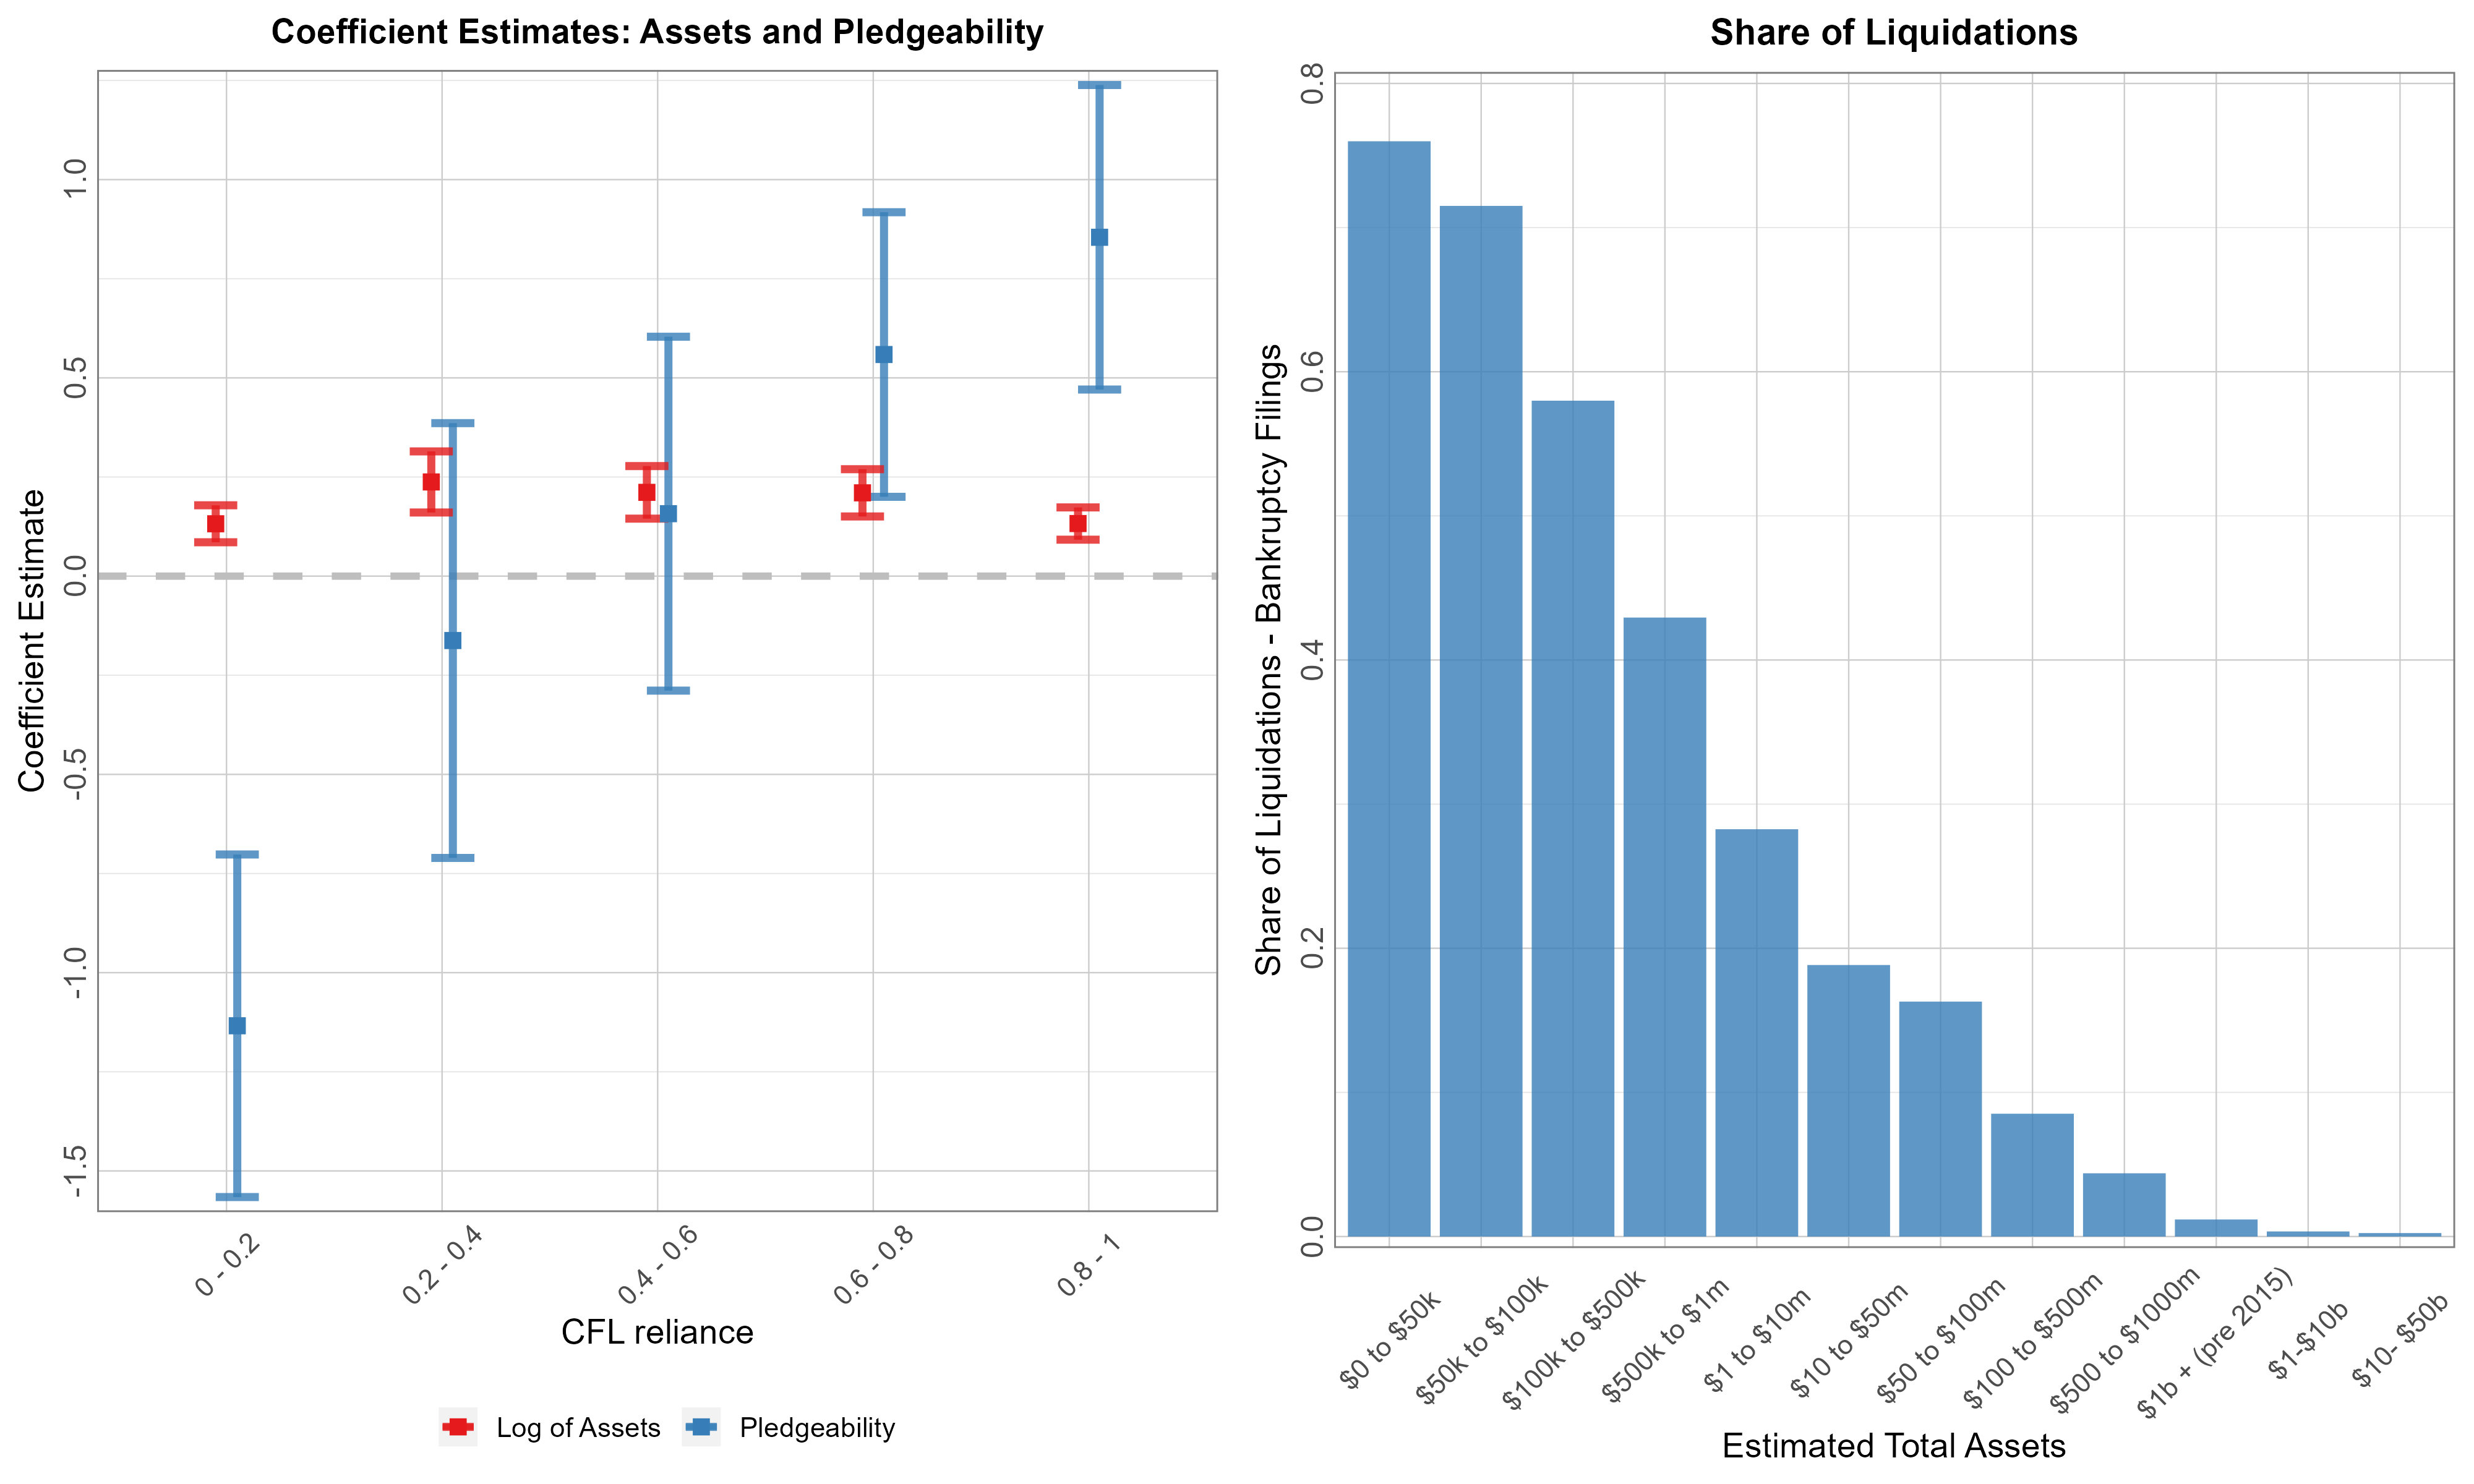
\includegraphics[width=1\textwidth]{C:/Users/szjud/OneDrive/Asztali gép/EBCs/CFL-git/Latex codes/Plots/mixplot.png}
     \footnotesize \justifying Panel A. present coefficient estimates from from the baseline specification for five groups of firms, categorized by their CF-share. The squares represent the coefficient estimates and the error bars show the 95\%  confidence intervals. Panel B. presents the liquidation decision across firm sizes. The bars show the number of bankrupt firms that got liquidated (Chapter 7.) over the total number of bankruptcy filings.
\end{figure}
\newpage 

\noindent To test the robustness of these results, I study these determinants in alternative specifications. Credit spreads have to be calculated manually, as a difference of the interest rate and the T-bill rate at the corresponding maturity. Calculating credit spreads such as this is subject to some uncertainty, therefore I consider the same models with interest rate as the dependent variable. In this case, I add maturity at the time of issueance to the control variables. These results are presented in table ... and ... of the appendix. Moreover, I repeat the debt-level regression on credit spreads without limiting the sample to new issuances - this regression is reported in table ... of the appendix. The qualitative predictions of these empirical models remain virtually unchanged in every alternative specification.

\subsection{Further Determinants of Credit Spreads\label{sec:credit spreads}}
Higher leverage has associated higher credit spreads in every specification, but this effects is somewhat larger for CF-based debt. This is intuitive as both the probability of default and lenders' exposure increases with debt. The logarithm of age is mostly associated with a significant, negative effect on credit spreads. This could reflect the importance of creditor and debtor relations, in decreasing the external finance premium. Somewhat surprisingly, age tends to have a stronger effect on asset-backed debt. The coefficient estimates the logarithm of the number of employees are not consistent across specifications. This variable have a limited economic impact, even when they are statistically significant, which indicates that assets are a sufficient measure of firms size. \vspace{3mm} \\
In each regression considered here, I include period and sector fixed effect - (the full specification is detailed in ... and ... in the appendix). Sector fixed effects have only a modest effect on credit spreads, which is partly due to also considering pledgeability as a separate variable. Moreover, I control for the credit ratings. These have large impact on the borrowing conditions. Consistent with the view that lender perception matters more in the case of CF-based debt, a worse rating is associated with strong increase in external finance premium. In contrast, for asset based debt contracts, credit spreads only react to credit ratings that are associated with high default risk.  \vspace{3mm} \\
Firms often rely on multiple debt contracts simultaneously, holding both cash flow-based and asset-based debt simultaneously. I measure firms' reliance to CF-based lending as the share of CF-based debt to total debt. This measure of `CF-share' is associated with lower spreads for CF-based borrowing and higher spreads for asset-based contracts. This highlights firms' self-selection into asset-based or CF-based borrowing. Firms with cheaper access to CF-based debt or costlier access to asset-based debt (due to some unobserved factors) tend rely more heavily on CF-based financing. \vspace{3mm} \\
Further inspection of CF-share, shows that only a small segment of overall market relies exclusively on one type of debt. That is, 35.7\% of firms use only asset-based debt, and 12.2\% rely solely on cash flow-based financing (CF-share of 0 and 1 respectively). The rest, 52.1\% of firms simultaneously hold both type of debt contracts. Since these are often the largest corporations, they correspond to 87.3\% of the market by the value assets and 90.3\% by the value of borrowing. This further highlights the limitations of classifying firms into two non-intersecting groups of borrowers, subject to asset-based or earnings-based frictions.

\subsection{Limitations}
Empirical analyses on the determinants of credit spreads must content with substantial limitations. First, credit spreads and debt financing strategy are jointly determined, meaning that firms' reaction to endogenous credit conditions, influences the interest rates they eventually face. Therefore, without relying on natural experiments, it is not possible to identify the effects of most determinants. Other potentially important determinants are not observable. In this paper, I argue that one such factors is the lenders' expectations that the firms would liquidate under financial distress. Assets specificity (Kermani and Ma, 2020) or the quality of accounting practices and court enforceability (Lian and Ma, 2021) are similarly elusive. To capture these effects, empirical analyses must rely on proxies or study highly specific datasets. The structural model discussed below makes up for some of these limitations. 

\section{Model outline} \label{sec:model}

In this section, I study the determinants of credits spreads in a partial equilibrium model. The model captures the effects of leverage, productivity and total asset. Firms also have a labour demand decision but number of employees does not directly impact credit conditions. To keep the model parsimonious, I do not consider differences in pledgeability or asset specificity. While this extension would be theoretically straightforward, introducing an additional state variable would increase computational burden.\footnote{Similarly, I do not differentiate between different sectors, as all firms produce the same homogenous consumption good and do not consider differences in credit ratings.} Instead, I focus on heterogeneity in liquidation probability, which was not previously considered by structural analyses in this context. Finally, I do not consider differences in firm age. To explore the effects of this variable, one would have to consider a Bayesian learning mechanism similar to Kochen (2022) as well as information asymmetries between creditors and lenders. This is beyond the scope of this paper.

\subsection{Firms and production \label{sec:production}}
Heterogeneous firms produce a homogeneous consumption good, using labour, $n$ and capital, $k$. Firms are competitive, and face a decreasing returns to scale production technology:
\begin{equation} \label{eq:prodf}
y = \varepsilon k^{\alpha}n^{\nu}, \ \ \ \ \alpha,\nu \in (0,1),  \ \nu + \alpha \in (0,1)
\end{equation}  
where $\varepsilon$ is the idiosyncratic productivity state. In the interest of keeping the notation simple, I omit firm subscripts. \vspace{3mm} \\
Firms own capital and investments are financed partly by financial wealth and partly by borrowing from a competitive lender. A firm can be described by the predetermined capital stock $k \in \mathbf{K} \subset \mathbf{R^{+}}$, debt\footnote{Firms may also decide to save in which case their debt towards the intermediary is negative.} $b \in \mathbf{B} \subset \mathbf{R}$ and current productivity $\varepsilon \subset \mathbf{R^+}$. Idiosyncratic productivity is a Markov chain on a finite set $\varepsilon \in \mathbf{E} \equiv \{ \varepsilon_1,...,\varepsilon_{N_{\varepsilon}} \}$ such that $ g_{ij} \equiv \Pr(\varepsilon'= \varepsilon_j|\varepsilon = \varepsilon) \geq 0$ and $\sum_{j=1}^{N_{\varepsilon}} g_{ij} = 1$ for each $i$. Moreover, it is stochastically monotone such that for any fixed $x$, $\Pr(\varepsilon' \leq x | \varepsilon = \varepsilon_i)$ is decreasing in $\varepsilon_i$. \vspace{3mm} \\
Production occurs before the realization of exit and entry decisions take effect, and optimal labor demand is independent of current debt. Therefore, every firm with the state vector at the beginning of the period $(k,\varepsilon)$ faces the same static optimization of labour: 
$$ \pi(k,\varepsilon) = \max_{n} \ \  \varepsilon k^{\alpha}n^{\nu} - wn - c$$
where $c$ is a fixed cost of participating in production, $w$ is equilibrium wage and the price of the consumption good is flexible and normalized to $1$. Optimization yields the policy function for labour demand, $n(\varepsilon,k)$ and optimal production $y(\varepsilon,k)$: 
\begin{equation} \label{eq:opt_emp_prod}
n(k,\varepsilon) = \left( \dfrac{ \nu \varepsilon k^\alpha}{w} \right)^{\frac{1}{1-\nu}} \hspace{15mm}
y(k,\varepsilon) = \varepsilon k^{\alpha} \left( \dfrac{\nu \varepsilon k^\alpha}{w} \right)^{\frac{\nu}{1-\nu}}
\end{equation}  
Firm profit function can be reformulated as: 
\begin{equation} \label{eq:profit}
\pi(k,\varepsilon) = y(k,\varepsilon) - wn(k,\varepsilon) - c = (1-\nu) y(k,\varepsilon) - c
\end{equation} 
Active firms own capital and make idiosyncratic investment decisions. Capital accumulation follows: 
\begin{equation} \label{eq:capital}
k' = (1-\delta)k + i
\end{equation} 
where $\delta$ is the depreciation rate and $i$ is investment. Capital adjustment is not subject to microeconomic frictions. Moreover, the lending schedule faced by individual firms depends only on future values of capital and debt, which firms may choose independently from current stocks. Hence, firms' financial position at any given period can be summarized by a cash on hand variable, $x \in \mathbf{X}$: 
\begin{equation} \label{eq:cash on hand}
    x = \pi(k,\varepsilon) + (1-\delta)k - b 
\end{equation}
The cash on hand and current productivity, $(x, \varepsilon)$ describe firms' current state. Hence, it is possible summarize the distribution of firms using the probability measure $\mu$ defined on the Borel algebra $A$, generated by the open subsets of the product spaces $ \mathbf{A} = \mathbf{X} \times \mathbf{E} $.  This reformulation reduces the computational burden the model. 


\subsection{Default and firm values \label{defaults}} 
Production takes places at the beginning of the period. Firms set their labour demand given $(k,\varepsilon)$, profits are realized and capital depreciates. After production, firms may experience an exogenous financial distress shock that is distributed uniformly across firms with probability $P_D$.\footnote{Introducing heterogeneity in default probabilities is not necessary to realize heterogeneity in debt contracts.} Under financial distress, the firm declares bankruptcy, which is associated with zero value regardless of the prior state or the eventual default resolution. Therefore, the continuation value is discounted with the probability of default: 
\begin{equation} \label{eq:V_0}
V_0(x,\varepsilon) = (1-P_\chi) V_1(x,\varepsilon)
\end{equation}
I define the indicator function $\chi_0$ which takes the value $1$ if the firm is reached by the insolvency shock and 0 otherwise. \vspace{3mm} \\
If the financial distress does not occur, the firm may decide to exit voluntarily. In this case, it retains the value of the depreciated capital stock net of debt service - i.e. the cash on hand. Let $V_1(x,\varepsilon)$ be the value of the firm before the voluntary exit decision is made. The firm chooses to exit if the current cash on hand exceeds the value associated with further production:
\begin{equation} \label{eq:V_1}
V_1(x,\varepsilon) = \max \Big\{ V_2(x,\varepsilon), \ x \Big\}
\end{equation} 
where $V_2(x,\varepsilon)$ is the value associated with further production. I define the indicator function $\chi_1$ which takes the value $1$ if the firms exits voluntarily and 0 otherwise. \vspace{3mm} \\
Firms that survive to the next period have access to external finance in the form of one-period debt contracts. For every unit of debt to be repaid in the next period, they receive $q$ units of output that may be allocated towards investment or distributed as dividends. It is possible to borrow against physical assets or future cash flows. These debt contracts are distinguished by different in-default payoffs. In particular, asset-based contracts are yield better pay-offs under liquidation and CF-based contacts extract more value under reorganization - I discuss this in detail in the following section. In every other respect, the two kind of debts are perfect substitutes, such that total debt is: $b = b^C+b^A$. Analogously to the empirical analysis, I define CFL reliance as: 
\begin{equation}
    \tau = b^C/(b^C+b^A).
\end{equation}
In summary, continuing firms choose future capital stock, $k'$, total future debt, $b'$ and debt financing strategy $\tau'$ to maximize the discounted sum of dividends, $d$ 
\begin{equation} \label{eq:dividends}
d = x - k' +  q(k',b',\varepsilon, \tau')b'
\end{equation} 
The value of further production is associated with the Bellman equation: 
\begin{equation} 
    V_2(x,\varepsilon) = \max_{k',b', \tau'} \left(x - k' +  q(k',b',\varepsilon, \tau')b' + \beta \E_{\varepsilon'|\varepsilon} V_0(x',\varepsilon') \right)
\end{equation}
subject to: 
\begin{equation}
x' = \pi(k',\varepsilon')+(1-\delta)k'-b' \hspace{5mm} \text{and} \hspace{5mm} d \geq 0
\end{equation}

\subsection{Financial intermediation}
\subsubsection{Default resolution}
Default resolution entails negotiations between the borrower and multiple creditors (with potentially conflicting interests), with the supervision of courts. Moreover, the negotiating parties' bargaining power may depend on the specific terms outlined in the contract. Hence, I do not attempt a comprehensive description of bankruptcy proceedings under different debt contracts. Instead, I focus on providing an accurate account of lenders' expected costs and pay-offs when debt is backed by assets or future cash flows. A substantial part of this analysis revolves around these costs and payoffs as they play a crucial role in shaping the debt schedule offered by lenders. \vspace{3mm} \\
Bankruptcy may be resolved either through liquidation or reorganization. Liquidation entails that the firm exits and the its undepreciated capital stock is liquidated at total cost of $(1-\phi_A)k$. The remainder is distributed between the household and the lender. Under reorganization, the household (who owns firms) pays the lender in order to keep to firm on the market. The total cost of reorganization is $ (1-\phi_C) V + \zeta$, where $\phi_C$ is the variable cost of reorganization and $\zeta$ denotes fixed costs discussed in section ... . \vspace{3mm} \\
Reorganization is efficient, such that it maximizes the remaining value (collateral or continuation) of the firm. Let $\chi_D = 1$ if the firm is liquidated under financial distress. Then,
\begin{equation} \label{eq:liquidation decision}
    \chi_D =  \mathds{1}(\phi_A (1-\delta) k  \  \geq \ \phi_C V_2(x,\varepsilon)- \zeta)  
\end{equation}

\subsubsection{The lender's problem}
The opportunity cost of lending to corporations is determined by the risk-free bond yields $q_0$. Since corporate lending is inherently risky, the competitive lender must charge a premium to break even. To set $q(k',b',\varepsilon, \tau')$ the lender considers the expected payoff under 3 distinct scenarios: \textit{a)} orderly repayment; \textit{b)} the firms is liquidated under financial distress; \textit{c)} the firms is reorganized under financial distress. From equation \ref{eq:liquidation decision}, it is possible to determine the probability that the firm will be liquidated under financial distress as follows: 
\begin{equation} \label{eq:liquidation probability}
    \gamma(k',b',\varepsilon) = \E_{\varepsilon'|\varepsilon}[\mathds{1}(\phi_A (1-\delta) k'  \  \geq \ \phi_C V_2(x',\varepsilon')- \zeta)]  
\end{equation}
It follows from the zero-profit condition that the debt schedule offered to firms is, 
\begin{equation} \label{eq:q}
    \begin{split}
        & q(k',b', \varepsilon, \tau')b' =  \beta \left[ (1-P_D)b' + \right. \\
        & \quad P_D \min \{b, \ \gamma \Pi_{liq}(k',b', \tau') +  \left. (1-\gamma) \E_{\varepsilon'|\varepsilon} \Pi_{reorg}(k',b', \varepsilon, \tau') \} \right] 
    \end{split}
 \end{equation}
where $\Pi_{liq}$ and $\Pi_{reorg}$ denote the expected payoff if the borrower undergoes liquidation and reorganization respectively. Also note that the minimum function indicates that the lender cannot recover more than the total value of the debt contract.  The next section discusses these in-default payoffs of the lender. 

\subsubsection{In-default payoffs}
Default resolution involves reallocating the remaining value (either collateral or continuation) of the firm in bankruptcy between lenders and the household. The debt financing strategy adopted prior to bankruptcy influences this redistribution.
Take asset-backed contracts first. When debt is secured against physical assets, the lender can enforce in-default payments by seizing and liquidating collateral. Thus, if the firm undergoes liquidation the lender can extract the full liquidation value $\phi_A (1-\delta) k$. When the borrower undergoes reorganization, the lender is protected by the `best interest of creditor' test (see section ...), which states that creditors cannot be worse off under the reorganization plan  than in case of the liquidation of the firm. Therefore, I assume that lender expects to extract the same $\phi_A (1-\delta) k$ payment after asset-backed debt contracts when borrower is reorganized. \vspace{3mm} \\
In contrast, CF-based debt is not secured by collateral, hence the lender can expect to retrieve only a small fraction $\kappa$ of the original liquidation value when the borrower is liquidated. Therefore, lenders must anticipate in-default payments chiefly from the reorganization of the borrower. Moreover, cash flow-based debt contracts often contain provisions that allow lenders to directly recover a portion of the going-concern value of the borrower. This allows the lender to retrieve some portion $\phi_C$ of the continuation value $V(k,b,\varepsilon)$, when the borrower undergoes reorganization. \\
\begin{table}[h!]
    \centering
    \begin{tabular}{l|cc}
        & Liquidation  & Reorganization \\  
       \midrule
      Asset based contract & $ \phi_A (1-\delta) k$  &  $ \phi_A (1-\delta) k$ \\
      CF based contract & $ \kappa \phi_A (1-\delta) k$ & $ \phi_C V(x,\varepsilon)$ \\ 
     \bottomrule
     \end{tabular}
    \caption{\small The lender's maximum potential payoffs under each default resolution-debt contract pair - gross of reorganization costs.} 
    \label{tab:lender payoffs}
\end{table}

\noindent With the information summarized in table \ref{tab:lender payoffs}, it is possible to outline the lender's expected payoff when the borrower undergoes liquidation or reorganization. In both cases, the lender's payoff is a determined not only by the value of the firm, but also the CFL reliance set before the realization of the bankruptcy. \vspace{3mm} \\
 First, let's consider the value retrieved after liquidation - $\Pi_{liq}$. The total liquidation value of the firm (i.e. the resale value of assets) is: $\phi_A (1-\delta) k'$. However, the lender can only retrieve this value for the  debt that is backed by collateral, which is $1-\tau$ share of the total debt. After the remaining $\tau$ share of the debt, the lender can only only seize $\kappa$ fraction of original liquidation value - see bottom-left of table \ref{tab:lender payoffs}. Taking stock, the lender receives:
\begin{equation} \label{eq:P_liq} 
   \Pi_{liq}(k,b,\tau) = (1-\tau) \phi_A (1-\delta) k +\tau \kappa \phi_A  (1-\delta) k
\end{equation}
Note that the value retrieved under liquidation does not depend on the realization of idiosyncratic productivity. The value not claimed by the lender is redistributed to the household in the form of lump-sum transfer.\footnote{This amounts to: $ \max \{\phi_A (1-\delta) k - b, \hspace{1mm} \tau (\phi_A-\phi_C) k  \} $.} \vspace{3mm} \\
CF-backed debt contracts allow lenders to extract $\phi_C$ portion of the continuation value. However, the reorganization process incurs a fixed cost, $\zeta$. When the lender expects in-default payments from reorganization, she considers that a portion of these costs may be incurred by her. In the following, I assume that lenders must pay $\tau$ share of this fixed cost.\footnote{This is an innocuous assumption. Lenders' expenses raise the costs of external finance premium of CF-based debt directly, whereas firms' costs raises the probability of resolving default via liquidation, which the raises costs of CF-based lending indirectly. Hence, the incidence of these costs has only a minimal effect on the external finance premium.} In accordance with the `best interest of creditors test', the lender expects to retrieve a payment that is equal to the liquidation value of the collateral after its asset-based debt. Taking stock, when the borrower undergoes reorganization, the lender receives:
\begin{equation}  \label{eq:P_reorg}
   \Pi_{reorg}(k,b,\varepsilon,\tau) = (1-\tau) \phi_A (1-\delta) k +\tau \min \{ 0, \ \phi_C V_2 (x, \varepsilon) - \zeta \}.
\end{equation}
To keep the model simple, I assume that reorganization entails that the household (the owner of the firm) pays the lender the lump-sum $\Pi_{reorg}$ to keep the firm going. In practice, extracting the continuation value may differ depending on the debt contract that is in place. When debt is secured against the entire corporate entity or equity, the lender can obtain ownership in the firm. In his case, it may directly seize future cash flows (and it gains direct influence on the liquidation decision). When the debt is unsecured, the lender has fewer devices to collect future cash flows. Nevertheless, in the absence of collateral, the lender's pay-offs chiefly depend on the continuation of the defaulted firm.\footnote{Corbae and D'Erasmo (2021) consider a Nash bargaining game for debt renegotiation. The threat of liquidation forces firms with high continuation value to agree to more generous terms of repayment. This implies that in default payments depend positively on the continuation value.} Therefore, in line with previous literature, I classify unsecured debt contracts as CF-based. 
\subsubsection{Optimal debt financing strategy}
It follows from the assumption that firms associate zero value with bankruptcy that debt financing strategy (i.e. the choice of $\tau'$) only affects firm values through the current external finance premium. Moreover, since firm value is increasing in $q(k',b',\varepsilon, \tau')$, for any $(k',b',\varepsilon)$ the optimal debt financing strategy coincides with the $\tau'$ that maximizes the inverse gross interest rate. Substituting equation \ref{eq:P_liq} and \ref{eq:P_reorg} into \ref{eq:q} and using that in the stationary equilibrium $q_0 = \beta$, we can express the optimal CFL reliance as follows:
\begin{equation} \label{eq:opt_tau}
    \begin{split}
        & \tau^*(k',b',\varepsilon) = \argmax_{\tau'} \ \  \frac{\beta}{b'} \Big{[} (1-P_D)b' \ +  \\
        & \quad  P_D \min \big{\{} b', \ \gamma \left((1-\tau') \phi_A (1-\delta) k' +\tau' \kappa \phi_A  (1-\delta) k' \right) \ +  \\
        & \quad (1-\gamma) \left( (1-\tau') \phi_A (1-\delta) k' +\tau' \left( \phi_C \E_{\varepsilon'|\varepsilon}V_2 (x', \varepsilon') - \zeta \right) \right) \big{\}} \Big{]} 
    \end{split}
 \end{equation}
With optimal CFL reliance, firms dynamic problem can be reformulated as, 
\begin{equation} \label{eq:V_2}
    V_2(x,\varepsilon) = \max_{k',b'} \left(x - k' +  q(k',b',\varepsilon)b' + \beta \E_{\varepsilon'|\varepsilon} V_0(x',\varepsilon') \right)
    \end{equation}
    subject to: 
    \begin{equation} \label{eq:cont_1}
    x' = \pi(k',\varepsilon')+(1-\delta)k'-b'; \hspace{10mm} d \geq 0;  \hspace{10mm} \tau' = \tau^*(k',b',\varepsilon)
    \end{equation}
    
\subsection{Firm dynamics}
In the previous sections, I defined the following indicator functions: $\chi_0 = 1$ if the insolvency shock materializes, $\chi_1 = 1$ if the firm is voluntarily liquidated, $\chi^D = 1$ if it is liquidated under financial distress. The combinations of these indicator functions describe the possible resolutions the debt contract, summarizted by \ref{table:indic}. Taking stock of liquidations, a firm may be liquidated voluntarily: $(1-\chi_0)\chi_1 = 1$ or under financial distress: $\chi_0\chi^D = 1$. These cases represent firms exits in the model. \vspace{3mm}\\
At every period, exits are balanced by a mass of entrants. These are endowed with a starting cash on hand and productivity drawn from the distribution $\Phi(x,\varepsilon)$. To reflect the fact that startup companies are typically asset-poor, this distribution is defined to yield low cash on hand on values relative to incumbent firms. The entry decision is described by equation \ref{eq:V_1}: potential entrants enter only if the continuation value is higher than their startup cost.\footnote{Entrants only start producing in the next period, hence their profits in the cash on hand variable is zero.} I define $\chi_e$ be equal to one if the potential entrant decides to enter and zero otherwise. 

\begin{table}[h!]
    \centering
    \begin{tabular}{|c|c|c|c|} 
    \hline
    Case &$\chi_0 $ - insolvency & $\chi_1, \ \chi_1^D$ - liquidation &  Outcome  \\ \hline
    1. & $\chi_0 = 0 $ &  $\chi_1 = 0$  & Repays debt, Continues \\
    2. & $\chi_0 = 0$ &  $\chi_1 = 1 $  & Repays debt, exits   \\
    3. & $\chi_0 = 1$ &  $\chi_1^D = 0$  & Insolvent, Reorganized  \\
    4. & $\chi_0 = 1$ &  $\chi_1^D = 1$ & Insolvent, Liquidated \\ 
    \hline
    \end{tabular}
    \caption{Possible debt contract resolutions in the model}
    \label{table:indic}
\end{table}
    
 \noindent Production takes place at the beginning of the period, therefore the measure, $\mu$ describes to the mass of active firms at any given time. Let $\overline{\mu}$ denote the measure of firms that are present at the end of the period. At each period, this evolves according to $ \overline{\mu} = (1-(1-\chi_0)\chi_1-\chi_0\chi^D) \mu + M \chi_{e} \ d \Phi$. The evolution of firm distribution then satisfies:
\begin{equation} \label{eq_firmdim} 
    \mu'(A) = \int \mathbf{I}_{(x', \varepsilon') \in A} g(\varepsilon'|\varepsilon) \ d \  \overline{\mu} (x,\varepsilon)
\end{equation}
for all Borel sets $A \subset  \mathbf{X} \times \mathbf{E} $ and where $g(\varepsilon'|\varepsilon)$ is the transition probability matrix idiosyncratic productivity. I summarize firm dynamics of firm distribution at the beginning of the period by the mapping $ \mu' =\Gamma(\mu)$.

\subsection{Households}\label{sec:hh}
Households choose consumption, $C$ labour, $L$ and non-contingent bonds, $B$ to maximize expected discounted utility - these yield the gross interest rate $1/q_0$. Moreover, households own all firms, which implies that they realize revenues and expenses from the production sector. On the revenue side, households receive dividends and the net wealth of firms that are liquidated voluntarily. On the expense side, households must endow entrants with starting capital, and re-buy firms that are reorganized by the financial intermediary. Moreover households receive lump-sum transfers $T$, that summarize costs and payoffs related to financial intermediation - these are summarized in section ... . These expenses and gains are pooled among households, hence the maximization problem:
\begin{equation} \label{eq:U_max}
V(B, \mu) = \max_{C,L,B'} U(C, 1-L) + \beta V(B', \mu')
\end{equation}  
subject to: 
\begin{multline} \label{eq:const_hh}
C + B + M \int  \chi_e (k-b) \ d \Phi(x,\varepsilon)  \leq wL + q_0 B' + T + \\  \int (1 - \chi_0) \chi_1 \ x \ d \mu(x,\varepsilon) + \int (1-(1-\chi_0)\chi_1-\chi_0\chi^D) \left( x - k'(x,\varepsilon) + qb'(x,\varepsilon) \right) d \mu(x,\varepsilon)
\end{multline} 
and given the evolution firm distribution measure: $\mu' = \Gamma(\mu)$. Transfers collect leftover capital value after involuntary liquidations and payment to the intermediary after reorganized firms. In total this amounts to 
\begin{multline*} \label{eq:T}
    T = \int \chi_0\chi^D  \max \{\phi_A (1-\delta) k - b, \hspace{1mm} \tau (\phi_A-\phi_C) k  \}  + \\
    \int \chi_0(1-\chi^D) \max \big{\{}b - [(1- \phi_v) V_2 (x, \varepsilon) + \zeta)], \\ (1-\tau)\phi_A(1-\delta)k + \tau V_2 (x, \varepsilon) + (1-\tau) [(1- \phi_v) V_2 (x, \varepsilon) + \zeta)]\big{\}} 
\end{multline*} 
Let the $C(b,\mu)$, $N(b,\mu)$, $B(b,\mu)$ be the policy functions for consumption, labour and next bond holdings in the next period. 

\subsection{Stationary equilibrium}\label{sec:eq}
The stationary competitive equilibrium can be described by the set of functions
$$(\mu, w, V_0, V_1, V_2, \chi^0, \chi^1, \chi^D, \chi^e, l,q,k,b,d, V_h, C, N, B)$$
such that: 
\begin{enumerate}[(i)]
\item Firms solve value maximization: $V_0$, $V_1$ solves \ref{eq:V_0}, \ref{eq:V_1} respectively and $V_2$ solves \ref{eq:V_2} and \ref{eq:cont_1} and the associated policy functions are $l$, for exiting firms and $(l,k,b,d,q)$ for entering and continuing firms
\item Households solve utility maximization: $V_h$ solves \ref{eq:U_max}-\ref{eq:const_hh} and the associated policy functions are $( C, N, B)$
\item Labour market clears: 
$$ N = \int n  \ d \mu (x,\varepsilon)  $$
\item Financial market clears:
 $$ B = \int b \ d \mu (x,\varepsilon) $$
\item Goods market clear: 
$$ C + I = \int y \ d \mu (x,\varepsilon)$$
where aggregate investment is the sum of investment carried out by continuing firms and startups minus the capital freed up due to voluntary and involuntary liquidations:
\begin{multline*} 
    I = \int (1-(1-\chi_0)\chi_1-\chi_0\chi^D)\left[ k' -(1-\delta)k \right] d \mu (x,\varepsilon) - \\
    \int \chi_0\chi^D (1-\delta) \phi_A k \ d \mu (x,\varepsilon) \int (1-\chi_0)\chi_1(1-\delta) k \ d \mu (x,\varepsilon)  + M \int \chi_e k \ d \Phi(x,\varepsilon) 
\end{multline*}
\item The distribution measure of active firms is stationary, $\Gamma(\mu) = \mu$ and prices $(w,q)$ are constant over time.
\end{enumerate}

\section{A1 - Bankruptcy practices \label{sec: qualitative analysis}}
\subsection{Default resolution frameworks \label{sec: default resolutions}}
When debt is secured against collateral, the lender expects to retrieve in-default payments by liquidating borrowers’ physical assets. The absence of such securities in case of cash flow-based contracts reflects creditors’ expectation that financial distress will be resolved through the reorganization of the borrower. Hence, asset-based debt contracts are consistent with liquidation, whereas cash flow-based contracts can be associated with the expected reorganization of the borrower.  \vspace{3mm} \\
However, the terms of debt contracts must be established ex-ante, whereas decisions concerning default resolution are made ex-post, only if financial difficulties arise. To better understand the determinants of creditors' expected, in-default payoffs under different debt contracts, it is worth discussing bankruptcy practices in more detail. In the following, I highlight some key characteristics of the US bankruptcy codes that will later inform the structural model. Appendix \ref{sec:A1} offers a more complete discussion of US bankruptcy procedures and also draws comparisons with the EU bankruptcy codes. \vspace{3mm} \\
\textit{a) The decision to reorganize or liquidate initially lies with the debtor, but lenders may enforce the conversion of the case under certain conditions.} Bankruptcy codes typically expect the debtor to first file for liquidation or reorganization - hence, the initial decision is in the hand of the debtor. Creditors may apply for the conversion of the default resolution, but this is approved only under special circumstances. Overall, the influence of a single lender over the default resolution is limited. Hence, unless the creditor deems that the probability of liquidation is zero, the terms of the debt contract must reflect the liquidation value of the borrower as well.\footnote{When the debt is secured against `substantially all assets', the lender becomes the owner of the entire corporate entity and it can make the liquidation decision himself. However, even in this case, the lender may find it more profitable to liquidate the company under certain conditions.}  \vspace{3mm} \\
\textit{b) Reorganizations must comply with the `best-interest-of-creditors' test.} This rule states that no dissenting creditor should be worse off under the proposed reorganization plan than it would be under the liquidation of the debtor. I refer to this principle as a basis to exclude scenarios in the structural model where asset-based borrowers undergo reorganization. In such cases, lenders can consistently expect to recover at least the liquidation value of the firm, making it unnecessary to consider this possibility when establishing conditions for asset-based lending. \vspace{3mm} \\
\textit{c) Special provisions to facilitate reorganization of SMEs}. Bankruptcy codes often attempt to alleviate the reorganization costs for small enterprises.\footnote{The EU directive allows member states to introduce special provisions to speed up and simplify the reorganization process for SMEs. The US bankruptcy code allow SMEs to file for a small business case (11 U.S.C. § 101(51C)) or under subchapter V of the Small Business Reorganization Act (SBRA), both of which are intended to streamline the reorganization process and reduce costs.} This is based on the recognition that these costs are often prohibitive for small enterprises. Despite the special provisions in place, SMEs are still far more likely to choose liquidation. I interpret this as evidence for the high fixed costs of the reorganization process. Continuing

\subsection{The fixed costs of lending against cash flows \label{sec:fixed costs}}
In the previous section, I emphasized that the empirical evidence points to substantial fixed costs of lending against future cash flows. This section identifies two possible sources of fixed costs: the costs of reorganization which materialize only under financial distress and monitoring costs that creditors must pay on an ongoing basis in order to maintain a realistic on the debtors' going-concern value. \vspace{3mm} \\
The reorganization process involves a lengthy negotiation between debtors, creditors, and courts, which imposes significant costs on the involved parties. When in-default payments are expected to be enforced via reorganization, the lender must take into account the legal, personnel and time expenses of this process. The costs of reorganization may fall on the debtor and the creditor as well. I summarize all fixed costs that materialize under the reorganization process with the parameter $\zeta_1$. \vspace{3mm} \\
Maintaining a cash flow-based debt contract may impose significant costs on the lender even in the normal course of business. Asset-based contracts only require occasional evaluations and audits of the borrower's assets. In contrast, cash flow-based contracts require that the lender carries out its `due diligence' on an ongoing basis. The apparatus to maintain this monitoring activity may impose significant expenses for the lender.\footnote{This type of cost shares some similarities with the costly state verification first proposed by Towsend (1979). Although this concept had significant influence in the macro-finance literature, it is typically not mentioned in relation to cash flow-based contracts.} I summarize costs of CF-based lending, that materialize regardless of financial distress, by $\zeta_2$. More generally, this could be thought of as all additional expenses lenders face on a regular basis, when they deviate from standardized asset-based contracts. In the structural model, these fixed costs represent significant limitation in access to cash flow-based contracts. 


\subsection{Bankruptcy frameworks in the US and EU  \label{sec:A1}}

The US Bankruptcy Code is structured into chapters, each corresponding to a different type of relief for debtors in financial distress. In particular, chapter 7 deals with liquidations and chapter 11 regulates the reorganization process. The European Union does not have a single bankruptcy code, but it has been working towards harmonizing insolvency proceedings across member states, based on the understanding that divergent insolvency laws create barriers across member states. As a result, the Harmonisation Directive\footnote{Directive (EU) 2019/1023 of the European Parliament and of the Council of 20 June 2019 on preventive restructuring frameworks, on discharge of debt and disqualifications, and on measures to increase the efficiency of procedures concerning restructuring, insolvency and discharge of debt.}  was published in June 2019, and member states are required to adopt the necessary legislative changes by July 2021 to comply with it. Although it does not completely standardize bankruptcy procedures, the directive outlines several principles that mirror the main features of chapter 7 and 11 of the US bankruptcy code. It represents a valuable piece of evidence for this discussion, as it collects the set of principles that legislators aim to institute in bankruptcy proceedings. \vspace{3mm} \\
Under both frameworks, the debtor is expected to file for insolvency – although creditors may petition the court to initiate bankruptcy proceedings against the debtor, this is not the norm. Hence, the decision to pursue reorganization or liquidation initially lies with the debtor. If the debtor decides to draft a reorganization plan, creditors may form committees and have their claims heard by courts. The European Union has a more debtor-friendly approach, meaning that creditors have less influence over the outcome of the proceedings, whereas the US system places more weight on the interest of the creditors. However, it is often the case that a debtor has numerous creditors, which limits the influence of any individual creditor over the specifics of the bankruptcy proceedings. \vspace{3mm} \\
One exception to this rule, is that no dissenting creditor should be worse off under the proposed reorganization plan than it would be in case of liquidation. The EU Directive refers this as ‘best-interest-of-creditors’ test in OJ L 172/27, art. 49; whereas the US bankruptcy code establishes this principle in 11 U.S. Code § 1129.  If the reorganization plan fails this test, it may not receive the necessary court approval (the dissenting creditor is entitled to vote against it). In the context of the model, this becomes relevant when an asset-based borrower decides to file for reorganization. The lender cannot receive a lower payoff than it expects to see from the liquidation of collateral (although it might have to pay some legal fees). Thus, from the point of view of the asset-based lender it does not matter if the borrower wishes to continue operating after the bankruptcy have been resolved. As discussed in section \ref{sec: qualitative analysis}, I abstract from these cases altogether.  \vspace{3mm} \\
Creditors have even less influence when a borrower seeks to resolve financial distress through liquidation of its assets - as it would be unrealistic to expect the firm to continue operating against the best judgement of its management. An important exception from this rule is when the debt is secured against the entire corporate entity. In this case, the creditor can take over the firm in case of default and may decide freely between reorganization and liquidation. Yet, cash flow-based lenders must take into account that in case of a default, they may only retrieve the liquidation value of the collateral.  This outcome could arise from mutual creditor-debtor agreement. Alternatively, it may reflect debtors' choice, possibly conflicting with the creditor's best interests. Hence, the risk premium on these loans will reflect the `Chapter 7 outcome’ too unless the lender deems that the probability of reorganization is negligible. 

\subsection{Data appendix \label{sec:A3}}
\subsubsection{Compustat and Capital IQ}
Compustat is a comprehensive, financial database maintained by S\&P Global. It offers standardized firm-level information on publicly traded companies compiled from financial statements, regulatory filings and other financial reports. I use the quarterly tables in Compustat North America which chiefly contains US and Canadian corporations. Moreover, I exclude financial corporations (SIC code 6000 to 6799) and utility providers (SIC code 4900-4999) from the sample. S\&P Capital IQ offers an extensive array of debt-level statistics. The two datasets can be connected via the unique firm a identifier (GVKEY), moreover Capital IQ covers most of the Compustat firms and yields consistent firm-level debt data after the aggregation of debt contracts. Although Capital IQ covers most major economies, I only focus on North American corporations, due to limitations introduced by Compustat.  \vspace{3mm} \\
Although both datasets provide high quality reports, reporting differences necessitate some manipulation of the data. Since monetary variables are often reported in the native currency, I bring all observations to USD. Moreover, Capital IQ reports data points in different units (units, thousands or millions). To be consistent to Compustat, I bring all observations to millions of units. It must also be ensured that each observation is uniquely identified by the combination of year, quarter, and debt ID. This may be violated for various reasons, for instance, debt facilities are often reported twice (once with the total accessible debt and once with the currently outstanding amount). Moreover, subsidiaries are also often included in the data. I exclude these to maintain observations at the highest consolidation level. \vspace{3mm} \\
In some instances, debt contracts go missing only to reappear a few quarters later. If this gap between observations is no more the 4 quarters, I use linear interpolation to fill up the data. These cases are relatively rare, they only amount to approximately 7\% of the total sample. To ensure the alignment of consistent observations, I aggregate debt-level data from CapitalIQ to the firm level and cross-reference it with the debt information reported by Compustat. I drop any observations where there is a disparity of more than 20\% between the two datasets. This amounts to around 8\% of the sample. The following tables summarize Compustat and Capital IQ variables, including their original names and definitions in these datasets.

\begin{table}[htbp]
\centering
\caption{Compustat variable definitions}
\label{tab:Compustat variable definitions}
\renewcommand{\arraystretch}{1.5} % Increase the vertical spacing of rows
\resizebox{\textwidth}{!}{%
\begin{tabular}{lp{5cm}p{7cm}} 
\toprule
Variable & Compustat Definition & Description \\
\midrule
Total debt & dlcq+dlttq & Long-Term Debt + Debt in Current Liabilities \\
Leverage & (dlcq+dlttq)/atq & Total debt / Total Assets \\
Collateral & ppentq+invtq+rectq & Total Property, Plant and Equipment (net) + Receivables + Inventory \\
Pledgeability & (ppentq+invtq+rectq)/atq & Collateral / Total Assets \\
Interest coverage & oibdpq / xintq & Operating income before depreciation / Interest related expenses \\
Investment & capxq-sppeq & Capital expenditures - Sale of Property \\
Investment rate & (capxy - sppey) / l.ppegtq & Investment / Lag of Total Property, Plant and Equipment (gross) \\
Equity & atq-ltq & Total assets / Total liabilities \\
Net debt & dlcq+dltq-chq & Total debt - Cash Holdings \\
Liquidity & chq/atq & Cash Holdings / Total Assets \\
Assets & atq & Total Assets (book value) \\
Liabilities & ltq & Liabilities (book value) \\
Revenue & revtq & Total quarter revenue \\
Employees & emp & Total number of employees (thousands) \\
Industry spec. & sic & SIC code \\
Credit rating & spcsrc & S\&P credit rating \\
Added value & revtq - cogsq & Total revenue - Input costs \\
Productivity & $\frac{revtq - cogsq}{ppegtq^{1/3} + emp^{2/3}}$ & Added value / Assets and Employees \\
Age & defined from Capital IQ & Current year - Year founded + 1 \\
\bottomrule
\end{tabular}
}
\end{table}

\newpage

\begin{table}[htbp]
\centering
\caption{Capital IQ Variables}
\label{tab:capital_iq_variables}
\begin{tabular}{ll}
\toprule
Variable & Capital IQ \\
\midrule
Loan value & dataitemvalue \\
Decimal of the value & unittypeId \\
Currency of issuance & issuedCurrencyId \vspace{3mm} \\
\multicolumn{2}{l}{\textbf{Used for classification}} \\
Description of the contract & capitalstructuredescription \\
Type of the debt contract & capitalstructuresubtypeid \\
Debt description in text & descriptiontext \\
Secured dummy & securedtypeid \\
Seniority & leveltypeid \vspace{3mm} \\
\multicolumn{2}{l}{\textbf{Firm-level aggregated variables}} \\
Total debt value & Sum of all contracts value \\
AB value & Sum of all AB debt \\
CF value & Sum of all CF debt \\
CF share & CF value / Total debt \\
\bottomrule
\end{tabular}
\end{table}

\end{document}